\section{МЕТОДЫ КЛАССИФИКАЦИИ ТЕКСТОВ НА БАЗЕ МАШИННОГО ОБУЧЕНИЯ}
Машинное обучение -- это набор методов, позволяющих на основе набора данных, называемого тренировочным, строить модели, позволяющие решать те или иные задачи без описания явного алгоритма их решения. Изменение параметров модели под решение конкретной задачи называется обучением. Существует три основных подхода к обучению:
\begin{enumerate}
    \item Обучение с подкреплением (Reinforcement learning);
    \item Обучение без учителя (Unsupervised learning);
    \item Обучение с учителем (Supervised learning).
\end{enumerate}

В задачах классификации используется подход <<Обучение с учителем>>, что характеризуется наличием метки о принадлежности одному или нескольким классам для каждого примера в обучающем наборе. Применительно к классификации текстов, первым шагом до обучения модели является преобразование текстового входа в численное представление в виде вектора. Простейшим примером такого алгоритма является метод bag-of-words, в котором вектор представляет частоту каждого слова в заранее определённом словаре. Основными моделями для решения задачи классификации текста являются:
\begin{enumerate}
    \item Наивный байесовский классификатор (Naive Bayes Classifier), основанный на теореме Байеса;
    \item Метод опорных векторов (Support Vector Machine или SVM), заключающийся в поиске гиперплоскости в многомерном пространтсве между точками, принадлежащими различным классам и являющимися отображением исходных данных в это пространство;
    \item Искусственные нейронные сети (Artificial Neural Networks), основанные на иммитации работы биологических нейронных сетей и позволящие извлекать высокоуровневую информацию из входных данных.  
\end{enumerate}

На сегодняшний день наиболее эффективной моделью для решения данной задачи являются искуственные нейронные сети, а конкретно глубокие нейронные сети (Deep Neural Networks).
\section{НЕЙРОННЫЕ СЕТИ}
Искуственная нейронная сеть (чаще называемая просто нейронной сети) -- вычислительная система, основанная на иммитации работы биологических нейронных сетей и обычно представляемая в виде графа. Простейшей нейронной сетью является однослойный перцептрон, представляющий собой один слой искусственных нейронов, называемый скрытым. Каждый искусственный нейрон умножает числовые входные данные на свой весовой коэффициент и применяет к результату смещение и активационную функцию. Математически это можно представить следующим образом:
\begin{equation}
    y = f(Wx + b),
\end{equation}  
где:
\begin{itemize}
    \item $x$ -- входные данные, вектор размерности $n$,
    \item $W$ -- матрица весов внутреннего слоя, размерность $n \times m$,
    \item $b$ -- вектор смещений внутреннего слоя, размерность $m$,
    \item $y$ -- выходные данные, вектор размерности $m$,
    \item $f$ -- активационная функция.
\end{itemize}

Примерами активационных могут служить следующие функции:
\begin{enumerate}
    \item Функция ReLU: $f(x) = \text{max}(0, x)$;
    \item Гиперболический тангенс: $f(x) = th(x) = \frac{e^x - e^{-x}}{e^x + e^{-x}}$;
    \item Логистическая функция: $f(x) = \sigma(x) = \frac{1}{1 + e^{-x}}$;
    \item Функция GELU: $f(x) = \frac{x[1 + \text{erf}(\frac{x}{\sqrt{2}})]}{2}$.
\end{enumerate}

Глубокими нейронными сетями называют искусственные сети, имеющие больше одного скрытого слоя, т.е. выход каждого скрытого слоя подаётся на вход следующему скрытому слою. Примерами таких нейронных сетей могут служить реккурентные нейронные сети (Reccurent Neural Networks или RNN), многослойные перцептроны (Multilayer Perceptron или MLP) или трансформеры.

Для оценки того, насколько предсказанный выход модели ($y_i$) отклоняется от требуемого ($\hat y_i$), вводится функция потерь. Таким образом обучение нейронной сети сводится к изменению параметров модели (весов $W$ и смещений $b$) так, чтобы функция потерь принимала минимальное значение. Изначально параметры инициализируются небольшими случайными числами. В качестве функций потерь могут использоваться следующие функции ($n$ -- количество примеров в тренировочном наборе данных):
\begin{enumerate}
    \item Средняя квадратичная ошибка (Mean Square Error или MSE): 
    \begin{equation}
        L = \frac{1}{n}\sum_{i = 1}^{n}\left(y_i - \hat y_i\right)^2;
    \end{equation}
    \item Перекрёстная энтропия (Cross-Entropy Loss): 
    \begin{equation}
        L = - \sum_{i = 1}^{n}\hat y_i \log \left(y_i\right);
    \end{equation}
    \item Функция потерь NLL (Negative Log-Likelihood): 
    \begin{equation}
        L = - \sum_{i = 1}^{n}\left( \hat y_i \log y_i + (1 - \hat y_i) \log (1 - y_i)\right).
    \end{equation}
\end{enumerate} 

Для минимизации функции потерь по обучающей выборке требуется вычислить градиент функции потерь по параметрам. Основным методом для вычисления является метод обратного распространения ошибки, позволяющий аналитически вычислить производную функции в точке. Метод основан на правиле вычисления производной сложной функции и автоматическом построении графа вычислений.

Обучение нейроной сети является итеративным процессом, каждая итерация которого является обработкой одного или нескольких примеров из обучающей выборки. Обработка всех примеров из обучающего набора называется эпохой. Каждая итерация состоит из четырёх этапов:
\begin{enumerate}
    \item Вычисление предсказания модели по входным данным (forward pass);
    \item Вычисление функции потерь;
    \item Вычисление градиента функции потерь по параметрам в точке (backward pass);
    \item Изменение параметров модели в заданном градиентом направлении.
\end{enumerate}

\section{ВЕКТОРНОЕ ПРЕДСТАВЛЕНИЕ ТЕКСТОВЫХ ДАННЫХ}
Основной проблемой в применении нейронных сетей для обработки естественного языка является представление текстовых данных в векторном виде (embeddings). Простейшим подходом для её решения является метод one-hot encoding, который заключается в следующем:
\begin{enumerate}
    \item Создаётся словарь, в котором содержатся все возможные слова;
    \item Каждому слову во входной последовательности ставится в соотвествие вектор размерности словаря, где в позиции, соответствующей этому слову в словаре, ставится единица, а во всех остальных ноль.
\end{enumerate}
Главной проблемой такого метода является размер получившегося вектора. Каждое слово кодируется вектором размерности всего словаря, что делает обработку закодированных таким образом данных очень затратной.

Более удачным и широко используемым методом для этого является токенизация. Токенизация представляет собой разбиение входного текста на части  (это могут быть символы, слова или части слов), называемыми токенами, и представление текста в виде последовательности номеров токенов в общем словаре. Таким образом, весь входной текст кодируется вектором, длина которого зависит только от длины входной последовательности. 

Однако такой способ всё ещё не отражает смысла и связи слов или частей слов между собой, поэтому следующим этапом в кодировании текстовой информации является обучение нейронной сети на основе входных данных в виде последовательности токенов для решения одной из задач языкового моделирования. Затем можно использовать получаемый из последнего скрытого слоя вектор в качестве закодированной информации высокого уровня и решать другие задачи, такие как классификация текста.
\section{КЛАССИФИКАЦИЯ ТЕКСТА}
Для решения задачи классификации текста необходим классификационный слой, отвечающий за создание выходных данных сети, которые представляют собой распределение вероятностей по классам. Он принимает в качестве входных данных значения, извлечённые предыдущими слоями, и применяет набор весов и смещений для получения набора оценок для каждого класса. При классификации текста задача может быть поставлена как задача с одним возможным классом для каждой последовательности (Single-label classification) и как задача с несколькими возможными классами для каждой последовательности (Multi-label classification).

В случае, если задача поставлена как Single-label classification, оценки, полученные моделью, преобразуются в вероятности с помощью функции softmax, которая гарантирует, что суммы вероятностей для всех классов равны 1. Затем класс с наибольшей вероятностью рассматривается как прогнозируемый класс для входных данных. Функция softmax определяется следующим образом:
\begin{equation}
    \sigma(z)_i = \frac{e^{z_i}}{\sum_{j=1}^{K} e^{z_j}},
\end{equation}
где:
\begin{itemize}
    \item $z$ -- вектор из K действительных чисел,
    \item $K$ -- размерность выхода предыдущего слоя,
    \item $i$ -- индекс, $1 \leq i \leq K$,
    \item $\sigma(z)_i$ -- i-я компонента вектора, полученного применением функции \texttt{softmax} к $z$.
\end{itemize}

В случае, если задача поставлена как Multi-label classification, оценки, полученные моделью, преобразуются в вероятности с помощью логистической функции $\sigma(x)$. В этом случае каждое полученное число в выходном векторе принимает значения от 0 до 1 и интерпретируется как вероятность принадлежности входного текста соответствующему классу. В зависимости от поставленной границы (например, считаем что последовательность принадлежит классу в том случае, если вероятность больше 90\%) входному тексту присваиваются соответствующие классы. 

Классификация намерений является частным случаем задачи классификации текста. В этом случае задача так же может быть поставлена как задача классификации с одним возможным классом и как задача классификации с несколькими возможными классами. Для того, чтобы выделяемые интенты было проще обрабатывать при использовании, решено поставить задачу как Single-label classification.
\section{ТРАНСФОРМЕРЫ}
Архитектура нейронной сети Transformer — это тип модели глубокого обучения, в которой используются механизмы внимания для 
обработки последовательных данных переменной длины. Модель состоит из нескольких блоков кодировщика (encoder) и декодировщика (decoder), 
каждый из которых содержит модуль Multi-Head Attention и сеть прямого распространения. Механизм Multi-Head Attention базируется на механизме Attention. Attention вычисляется по следующей формуле:
\begin{equation}
    \text{Attention} = \text{softmax}\left(\frac{QK^T}{\sqrt{d_k}}\right)V,
\end{equation}
где:
\begin{itemize}
    \item $Q = X W_Q$ -- вектор размерности $d_k$,
    \item $K = X W_K$ -- вектор размерности $d_k$,
    \item $V = X W_V$ -- вектор размерности $d_v$,
    \item $X$ -- входной вектор размерности $d_{model}$,
    \item $W_Q$ -- параметры модели, матрица размерности $d_{model} \times d_k$,
    \item $W_K$ -- параметры модели, матрица размерности $d_{model}\times d_k$,
    \item $W_V$ -- параметры модели, матрица размерности $d_{model} \times d_v$. 
\end{itemize}
Multi-Head Attention является расширением механизма Attention и вычисляется по формуле
\begin{equation}
    \text{MultiHead} \left(Q, K, V\right) = \text{Concat}(\text{head}_1, \text{head}_2, ..., \text{head}_h)W^O,
\end{equation}
где каждый $\text{head}_i$ вычисляется параллельно по следующей формуле:
\begin{equation}
    \text{head}_i = \text{Attention}(QW_i^Q, KW_i^K, VW_i^V),
\end{equation}
где:
\begin{itemize}
    \item $W_i^Q$ -- матрицы параметров модели размерностью $d_{model} \times d_k$,
    \item $W_i^K$ -- матрицы параметров модели размерностью $d_{model} \times d_k$,
    \item $W_i^V$ -- матрицы параметров модели размерностью $d_{model} \times d_v$,
    \item $W^O$ -- матрица параметров модели размерностью $hd_v \times d_{model}$,
    \item $d_k = d_v = d_{model} / h$,
    \item $d_{model}$ -- размерности внутренних слоёв модели.
\end{itemize}

Multi-Head Attention позволяет модели взвешивать важность различных частей входной последовательности, в то время как сеть прямой связи применяет к входным данным нелинейные преобразования. Кроме того, архитектура модели позволяет обрабатывать несколько примеров параллельно за счёт упаковки входных векторов $X$ в матрицу размерности $d_b \times d_{model}$, где $d_b$ -- количество примеров, обрабатываемых одновременно. Помимо этого, важным элементом является кодирование позиции токенов во входной последовательности, что также учитывается в моделях архитектуры Transformer. Выход кодировщика подается в декодировщик, который генерирует окончательную выходную последовательность на основе взвешенных комбинаций выходов этого кодировщика и собственного предыдущего выхода декодировщика (рисунок \ref{transformer:image}) \cite{transformers}.
\begin{figure}[H]
    \begin{center}
        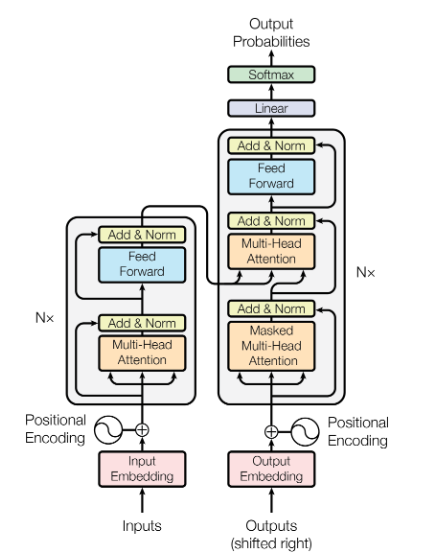
\includegraphics[width=.6\linewidth]{transformers.png}
        \caption{Архитектура модели класса Transformer}
        \label{transformer:image}
     \end{center}
\end{figure}

В контексте классификации текста модели класса Transformer могут использоваться для кодирования входного текста в векторное представление 
фиксированной длины, которое затем может быть передано в классификатор для прогнозирования метки класса. Обычно это делается с помощью 
предварительно обученной модели класса Transformer (такой как BERT или GPT) для кодирования текста, а затем добавления 
классификационного слоя и точной настройки модели на размеченном наборе данных с использованием подхода 
<<обучение с учителем>> (Supervised learning). 

\section{МОДЕЛИ}
Для исследования были выбраны следующие модели:
\begin{itemize}
    \item BERT;
    \item RoBERTa;
    \item DistilBERT;
    \item ALBERT;
    \item ELECTRA;
    \item OPT.
\end{itemize}

Это связано с тем, что эти архитектуры являются наиболее популярными при обработке естественного языка, в частности при классификации текстов, что связано с их эффективностью в этих задачах, а также небольшими затратами на обучение моделей данных архитектур. Для каждой архитектуры была взята модель базового размера. 
\subsection{BERT}
BERT (Bidirectional Encoder Representations from Transformers) является одной из самых популярных и используемых архитектур класса Transformer. BERT — это encoder-only (т.е. из transformer-блока encoder+decoder остаётся только encoder) двунаправленная модель, предобученная изначально на задачах размаскирования (Masked Language Modeling или MLM) и предсказания следующего предложения (Next Sentence Prediction или NSP).
Задача MLM заключается в следующем: 15\% токенов в исходной последовательности выбираются для возможной замены, 80\% заменяются токеном \texttt{[MASK]}, 10\% остаются без изменений, оставшиеся 10\% заменяются на случайный токен в словаре. В качестве целевого примера используется изначальная последовательность. Задача NSP ставится следующим образом: в качестве входной последовательности подаются два сегмента, разделённые специальным токеном \texttt{[SEP]}, а модель предсказывает, являются ли они последовательными сегментами из одного текста или нет. Обе задачи при обучении BERT решаются одновременно \cite{bert}.

\subsection{RoBERTa}
RoBERTa (Robustly optimized BERT approach) – версия модели BERT, для которой провели дополнительные исследования для улучшения качества итоговой модели. Результатами такого исследования стали следующие решения на этапе обучения модели:
\begin{itemize}
    \item Шаблон маскирования формируется динамически перед формированием набора примеров для одного шага оптимизации, тогда как в оригинальной модели шаблон маскирования формируется один раз перед обучением;
    \item Вместо сегментов текста подавались целиком предложения;
    \item Из итоговой функции потерь исключили добавку для задачи NSP, при этом данные формируются тем же образом (предложения подаются парами);
    \item Увеличили размер набора для одного шага оптимизации;
    \item Увеличили количество данных для обучения.
\end{itemize}
Такой подход позволил получить более эффективную модель на выходе \cite{roberta}.

\subsection{DistilBERT}
DistilBERT (Distilled BERT) — версия BERT, к которой применили процесс дистилляции знаний на фазе обучения, что позволило уменьшить размер модели на 40\%, сохранив при этом 97\% эффективности изначальной модели. Процесс заключается в том, чтобы сделать модель с меньшим количеством весов за счёт уменьшения количества слоёв относительно оригинальной модели в 2 раза, сохраняя ту же архитектуру, и при обучении сделать добавку в функцию ошибки, которая заставляет модель выдавать те же ответы, что и оригинальная модель. Обучалась модель на тех же данных и на той же задаче, что и BERT \cite{distilbert}.

\subsection{ALBERT}
ALBERT (A Lite BERT) –  ещё одна версия BERT, в архитектуру которой внесли изменения, позволяющие сократить количество параметров модели 
при сохранении её эффективности, что сокращает затраты на её обучения и использование. Для достижения этого эффекта были внесены следующие 
архитектурные изменения: 
\begin{enumerate}
    \item Добавлен дополнительный слой перед скрытыми, для того чтобы отделить размер входной последовательности от размера скрытого слоя;
    \item В разных слоях используются одни и те же веса, что позволяет уменьшить занимаемую моделью память при незначительном снижении качества модели.
\end{enumerate}
Помимо этого задачу NSP сменили на задачу предсказания порядка предложений (Sentence Order Prediction или SOP), что также улучшило качество итоговой модели. Задача SOP отличается от NSP подбором примеров: если в качестве негативных примеров в NSP брались сегменты из разных текстов, то в SOP в качестве негативных примеров используются последовательные сегменты текста, которые поменяли местами \cite{albert}.

\subsection{ELECTRA}
ELECTRA (Efficiently Learning an Encoder that Classifies Token Replacements Accurately) – модель, схожая в своей архитектуре с BERT. 
В отличие от оригинальной модели, обучение ELECTRA происходило следующим образом: есть две модели (Generator и Discriminator), которые обучаются вместе. 
Generator получает на вход последовательности с маскированными токенами и пытается их восстановить, 
а Descriminator пытается определить, какие токены в последовательности являются сгенерированными моделью-генератором, а какие изначально находились в последовательности. 
После обучения Generator не используется, а в Discriminator меняется выходной слой под нужную задачу, после чего дообучается уже на новой задаче. 
Такой метод обучения позволил уменьшить размеры модели, а соответственно и затраты на её обучение, при этом улучшив её эффективность
\cite{electra}.

\subsection{OPT}
OPT (Open Pre-trained Transformers) - это decoder-only модель, которая по сути является аналогом GPT-3 (Generative Pre-trained Transformers), 
но отличается от неё меньшими затратами на обучение и тем, что является полностью доступной, в отличие от GPT-3. Модель обучена на большом 
количестве данных изначально для генерации текста \cite{opt}.

\section{МЕТРИКИ}
Основными метриками для оценки моделей классификации являются accuracy (точность) и $F_1$. Изначально обе метрики вводятся для оценки качества 
решения задачи бинарной классификации, однако в задаче с большим количеством классов можно также использовать эти метрики: точность в том же виде,
а $F_1$ с некоторыми изменениями.

Accuracy показывает количество правильно данных моделью ответов и высчитывается по следующей формуле:
\begin{equation}
    \text{Accuracy} = \frac{K}{N},
\end{equation}
где:
\begin{itemize}
    \item $K$ -- количество правильно предсказанных примеров,
    \item $N$ -- общее количество примеров в выборке.
\end{itemize}
Однако такая метрика не является исчерпывающей, так как она не учитывает дисбаланс классов в выборке.

Более строгой и репрезентативной в данном случае является $F_1$-метрика. Она учитывает не только количество правильных ответов, но и 
ошибки первого и второго рода. В задаче бинарной классификации $F_1$ высчитывается по следующей формуле:
\begin{equation}
    F_1 = \frac{TP}{TP + \frac{FP + FN}{2}},
\end{equation}
где:
\begin{itemize}
    \item $TP$ -- количество правильно предсказанных меток первого класса,
    \item $FP$ -- количество неправильно предсказанных меток первого класса или ошибок первого рода (примеру второго класса присваивается метка первого класса),
    \item $FN$ -- количество неправильно предсказанных меток второго класса или ошибок второго рода (примеру первого класса присваивается метка второго класса).
\end{itemize}

Для задачи с большим количеством классов $F_1$ расширяется двумя способами:
\begin{enumerate}
    \item Macro $F_1$;
    \item Micro $F_1$.
\end{enumerate}

Macro $F_1$ высчитывается как среднее $F_1$ по каждому классу, а в micro $F_1$ составляющие $TP$, $FP$, $FN$ высчитываются как сумма 
соответствующих величин по каждому классу.  
